%iffalse
\let\negmedspace\undefined
\let\negthickspace\undefined
\documentclass[journal,12pt,onecolumn]{IEEEtran}
\usepackage{cite}
\usepackage{amsmath,amssymb,amsfonts,amsthm}
\usepackage{algorithmic}
\usepackage{graphicx}
\usepackage{textcomp}
\usepackage{xcolor}
\usepackage{txfonts}
\usepackage{listings}
\usepackage{enumitem}
\usepackage{mathtools}
\usepackage{gensymb}
\usepackage{comment}
\usepackage[breaklinks=true]{hyperref}
\usepackage{tkz-euclide} 
\usepackage{listings}
\usepackage{gvv}                                        
%\def\inputGnumericTable{}                                 
\usepackage[latin1]{inputenc}                                
\usepackage{color}                                            
\usepackage{array}                                            
\usepackage{longtable}                                       
\usepackage{calc}                                             
\usepackage{multirow}                                         
\usepackage{hhline}                                           
\usepackage{ifthen}                                           
\usepackage{lscape}
\usepackage{tabularx}
\usepackage{array}
\usepackage{float}
\usepackage{multicol}
\usepackage{subcaption}

\newtheorem{theorem}{Theorem}[section]
\newtheorem{problem}{Problem}
\newtheorem{proposition}{Proposition}[section]
\newtheorem{lemma}{Lemma}[section]
\newtheorem{corollary}[theorem]{Corollary}
\newtheorem{example}{Example}[section]
\newtheorem{definition}[problem]{Definition}
\newcommand{\BEQA}{\begin{eqnarray}}
\newcommand{\EEQA}{\end{eqnarray}}
\newcommand{\define}{\stackrel{\triangle}{=}}
\theoremstyle{remark}
\newtheorem{rem}{Remark}


% Marks the beginning of the document
\begin{document}
\bibliographystyle{IEEEtran}
\vspace{3cm}

\title{NCERT-11.16.4.5.1}
\author{S. Sai Akshita - EE24BTECH11054}
\newpage
\maketitle
\bigskip

\renewcommand{\thefigure}{\theenumi}
\renewcommand{\thetable}{\theenumi}
\textbf{Question:} Out of 100 students, two sections of 40 and 60 are formed. If you and your friend
are among the 100 students, what is the probability that you both enter the same section?\\
\textbf{Solution:} For both the students to be in the same section, there are 2 possible cases:\\
\begin{enumerate}
    \item Both are present in section A (Consisting of 40 students)=$P\brak{A_1\cap A_2}$. \\
    \item Both are present in section B (Consisting of 60 students)=$P\brak{B_1\cap B_2}$.
\end{enumerate}

Each student is independently assigned to one of the two sections. Since there are 40 spots in one section and 60 in the other, the probability that students 1 and 2 is assigned to section A is:
\begin{align}
    P\brak{A_1} &= \frac{40}{100} = 0.4\\
    P\brak{A_2/A_1} &= \frac{39}{99} =0.393
\end{align}
Similarly, the probability of being assigned to the second section (size 60) is:
\begin{align}
P\brak{B_1} &= \frac{60}{100} = 0.6\\
P\brak{B_2/B_1} &= \frac{59}{99} = 0.595
\end{align}

Evaluating probabilities for both the cases:
\begin{align}
    P\brak{\text{Both in 40}}&=P\brak{A_1\cap A_2}\\
    &=P\brak{A_1}\times P\brak{A_2/A_1}\\
    &= \frac{40}{100} \times \frac{39}{99}
\end{align}

\begin{align}
    P\brak{\text{Both in 60}}&=P\brak{B_1\cap B_2}\\
    &=P\brak{B_1}\times P\brak{B_2/B_1}\\
    &= \frac{60}{100} \times \frac{59}{99}
\end{align}

Now summing both cases for total probability:

\begin{align}
P\brak{\text{Same Section}} = P\brak{A_1\cap A_2}+P\brak{B_1\cap B_2}
&= \brak{ \frac{40}{100} \times \frac{39}{99} } + \brak{ \frac{60}{100} \times \frac{59}{99} }\\
P\brak{\text{Same Section}} \approx 0.5152 \approx 0.52
\end{align}
\textbf{Solution using Discrete Random Variable:}
Let $ X $ be a discrete random variable representing the number of students (out of you and your friend) assigned to the first section of 40 students.

Since each student is independently placed in either of the two sections, $ X $ can take values $0, 1,$ or $2$, where:
\begin{itemize}
    \item $X = 0 $: Neither you nor your friend is in the first section (both in the second section).
    \item $X = 1 $: Exactly one of you is in the first section, and the other is in the second section.
    \item $ X = 2 $: Both you and your friend are in the first section.
\end{itemize}
Since each of them are independently placed in a section, $X$ follows a Binomial Distribution with parameters $n = 2 $ and $ p = 0.4 $,

\begin{align}
X \sim \text{Binomial}\brak{2, 0.4}
\end{align}

The Probability Mass Function (PMF) of a Binomial random variable is:

\begin{align}
P\brak{X = k} = \binom{2}{k} p^k \brak{1 - p}^{2-k}, \quad k = 0,1,2
\end{align}
where $p = 0.4 $ and $ 1 - p = 0.6 $.
We want the probability that both students are in the same section. This happens in two cases:
\begin{itemize}
    \item Both are in section A ($ X = 2 $).
    \item Both are in section B ($ X = 0 $).
\end{itemize}
Now, computing the probabilities:
\begin{align}
P\brak{X = 0} &= \binom{2}{0} \brak{0.4}^0 \brak{0.6}^2 = 1 \times 1 \times 0.36 = 0.36\\
P\brak{X = 2} &= \binom{2}{2} \brak{0.4}^2 \brak{0.6}^0 = 1 \times 0.16 \times 1 = 0.16
\end{align}
Thus, the required probability is:
\begin{align}
P\brak{X = 0} + P\brak{X = 2} = 0.36 + 0.16 = 0.52
\end{align}
Thus, the probability that both you and your friend end up in the same section is $52\%$.


\begin{center}
    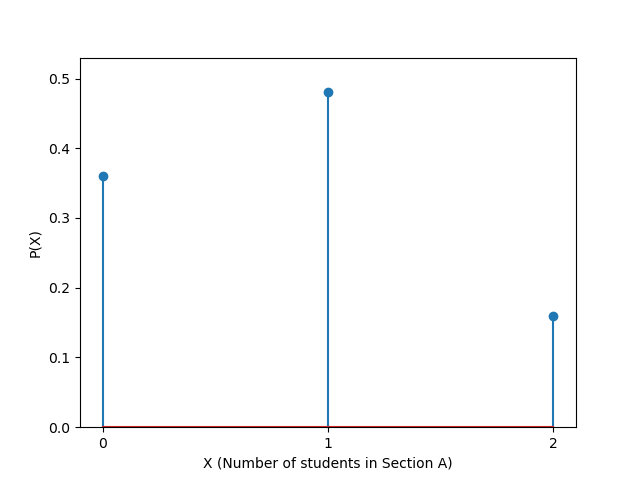
\includegraphics[width=\columnwidth]{figs/probability.png}
\end{center}








\end{document}
